\section{Buildroot}
\paragraph{}
Buildroot est un framework permettant de compiler un linux embarqué. Pendant longtemps buildroot a été la référence. Il propose, via un outil graphique, de paramétrer son système en fonction de ses besoins.

\begin{figure}[!h]
    \center
    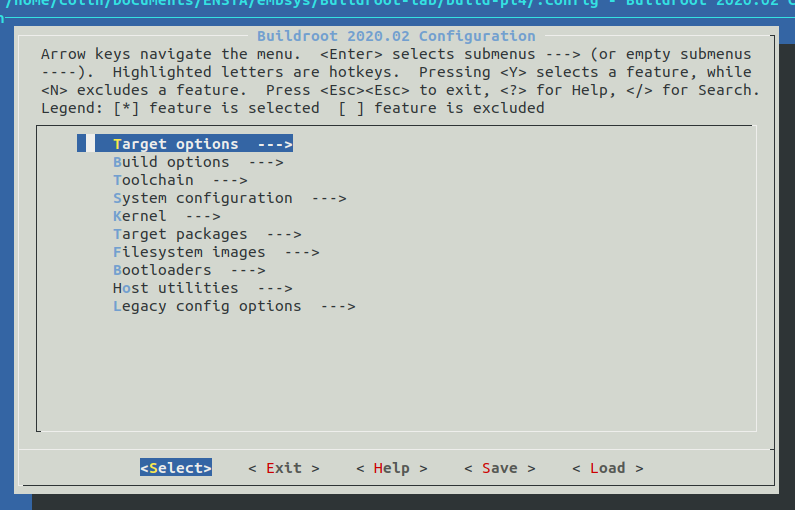
\includegraphics[width=10cm]{Images/menuconfig.png}
    \caption{Menu obtenu par ma commande \$make menuconfig}
\end{figure}

\paragraph{}
L'ajout de code métier ou de packages non présents dans le menu est bien sûr possible.
Cependant avec la diversification des applications et les temps de développements courts, les développeurs ont de plus en plus recours à des modules externes. Et c'est là que Buildroot montre ses limites. Chaque mise à jour implique une recompilation de tout le système, entraînant une certaine lourdeur. Il est à noter que Buildroot utilise l'outil GNU-Make, et n'utilise pas de fait des threads (il utilise bien entendu tous les coeurs du processeur à disposition), fonctionnalité dont est pourvu Yocto qui peut simultanément télécharger, configurer et compiler, optimisant ainsi le processus.



